
\chapter{Basic notions}

\label{seq:basic}

\section{Camera geometry}

\begin{figure}[t]
  \begin{center}
    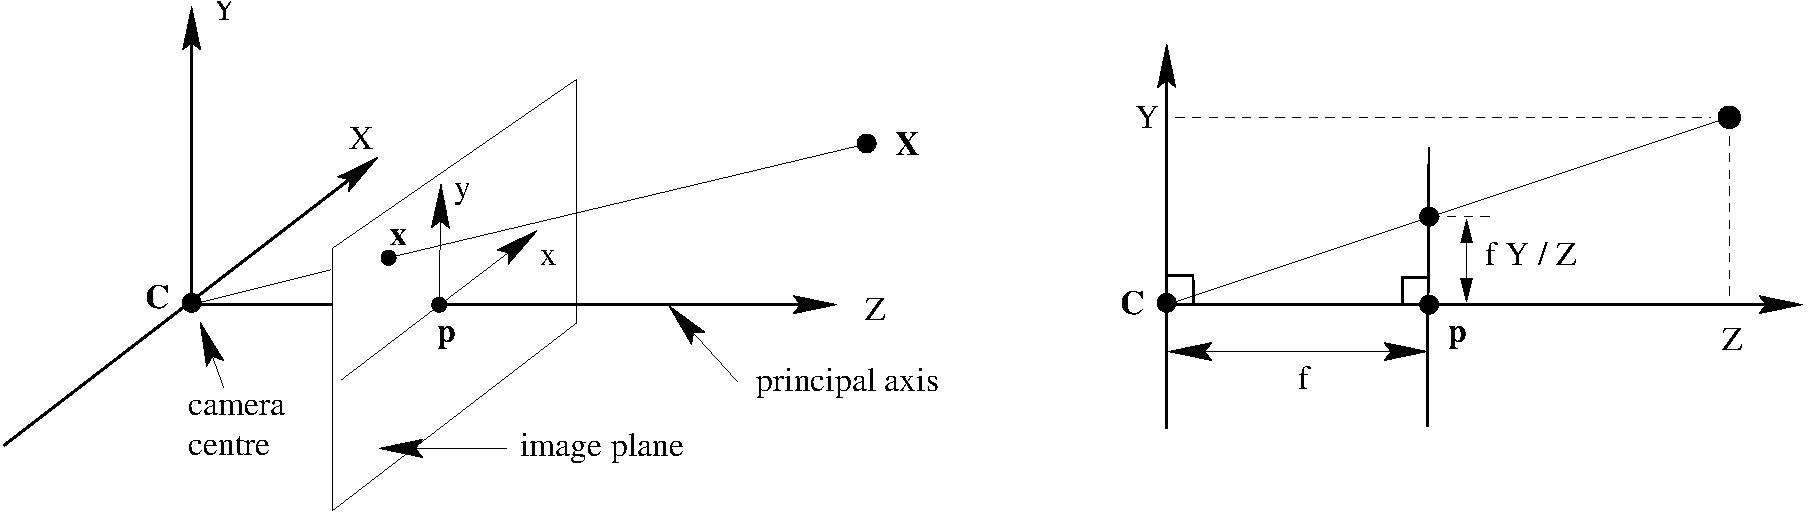
\includegraphics[width=\linewidth]{cammodel.pdf}
    \caption[Projective camera model]{Projective camera model. Courtesy of~\cite{HartZiss}}
    \label{cameramodel}
  \end{center}
\end{figure}

The book~\cite{HartZiss} describes camera geometry, the main topic of this thesis, in chapter 6. All needed preliminaries are also well described in chapters 1-5 of the book. In the next two sections we very briefly summarize and recapitulate the topic. We follow the notation of~\cite{HartZiss}.

\subsection{Single camera geometry}

The most convenient way of representing points in 3D or 2D space while dealing with camera geometry is using corresponding projective spaces.

\begin{defn}
Given a linear vector space $\R^n$, a \textit{projective space} $\Proj^{n-1}$ could be defined as a factorization of the linear space by a relation $\sim$: \[\mathbf{x}_1 \sim \mathbf{x}_2 \iff (\exists \lambda \in \R\backslash\{0\} \; \mathbf{x_1}=\lambda \mathbf{x_2}).\]

The zero point is also excluded from projective space.
\end{defn}


A point $\mathbf{X}_i=\mat{ccc}{x & y & z}^\T$ from 3D linear space $\mathbb{R}^3$  can be though of as a point $\mathbf{X}'=\mat{cccc}{x & y & z & 1}^\T$ from 3D projective space $\Proj^3$. Similarly, a point $\mathbf{X}'=\mat{cccc}{x & y & z & f}^\T$ can be converted back to the point $\mathbf{X}=\mat{ccc}{\frac{x}{f} & \frac{y}{f} & \frac{z}{f}}^\T$ unless $f$ is zero. Because of this possible conversion we will frequently refer to the same geometrical point as belonging to projective space $\Proj^{n-1}$ as well as linear space $\R^n$ simultaneously. 

\begin{defn}
A projective line is a line of points in projective space $\Proj^{n}$. Conveniently, it can be also represented by a point from the space  $\Proj^{n}$. For example, a line in projective plane $a x + b y + f c = 0$, which corresponds to the line $a x + b y + c = 0$ in  real plane, can be written as a point $\mathtt{l} = \mat{ccc}{a & b & c}^\T$.
\end{defn}


The Fig. \ref{cameramodel} shows an essential concept of projecting points from world (3D) space to image (2D) space. This projection can be described as a linear operation in corresponding projective spaces. 

The projection operator is given by camera parameters, which can be divided in two groups - extrinsic and intrinsic parameters.
We next define essential intrinsic parameters. 

\begin{defn}
\textit{The principal axis}, also \textit{optical axis}, is the line passing through camera center and perpendicular to the image plane.
\end{defn}

\begin{defn}
\textit{The principal point} $\mathbf{p}=\mat{ccc}{p_x & p_y & 1}^\T$ is the point lying at the intersection  of image plane and principal axis.
\end{defn}

\begin{defn}
\textit{The focal length} $f$ is the distance from the camera center to the principal point. 
\end{defn}

Camera intrinsic parameters are can be formed into camera calibration matrix.

\begin{defn}
\textit{A iatrix\footnote{Throughout this work we assume unity aspect ratio and zero skew.}} $\mathtt{K}$ is a matrix of the form \[ \mathtt{K} = \mat{ccc}{f & 0 & p_x \\ 0 & f & p_y \\ 0 & 0 & 1}. \] 
\end{defn}

If we assume that the camera center is the world space zero point, principal axis coincide with $Z$ axis, and image space axes $x$, $y$ are aligned with world space axes $X$, $Y$ (true for the Fig. \ref{cameramodel}), we can project 3D points with only camera intrinsics. The projection from $\R^3$ to $\Proj^2$ image plane is given by $\mathbf{x}_i = \mathtt{K} \mathbf{X}_i $.

Extrinsic parameters of a camera $i$ are described by a rotation matrix in the world space $\mathtt{R}_i$ describing camera orientation and the camera center point  $\mathbf{C}_i$ in the world space.  
Given extrinsic and intrinsic parameters, we can construct the full projection matrix.

\begin{defn}
The camera \textit{projection matrix} $\mathtt{P}_i$ can be constructed from camera parameters and projects points $\mathbf{X}_i$ from world space $\Proj^3$ to the image plane $\Proj^2$: \[\mathbf{x}_i = \mathtt{P} \mathbf{X}_i =  \mathtt{K} \mathtt{R} [ \mathtt{I} | -\mathbf{C} ] \mathbf{X}_i \].

\end{defn}


\subsection{Epipolar geometry} 
Epipolar geometry, one of the key topics of this thesis, is a geometry of two cameras seeing the same 3D object. 

This section is described in depth in chapter 9 of~\cite{HartZiss}. As a slight deviation from the notation of Hartley and Zisserman, cameras and respective image points are indexed with numbers, e.g., $\mathbf{x}_1$, $\mathbf{x}_2$ and not $\mathbf{x}$, $\mathbf{x}'$ respectively.


\begin{figure}[t]%
    \centering
    \subfloat{{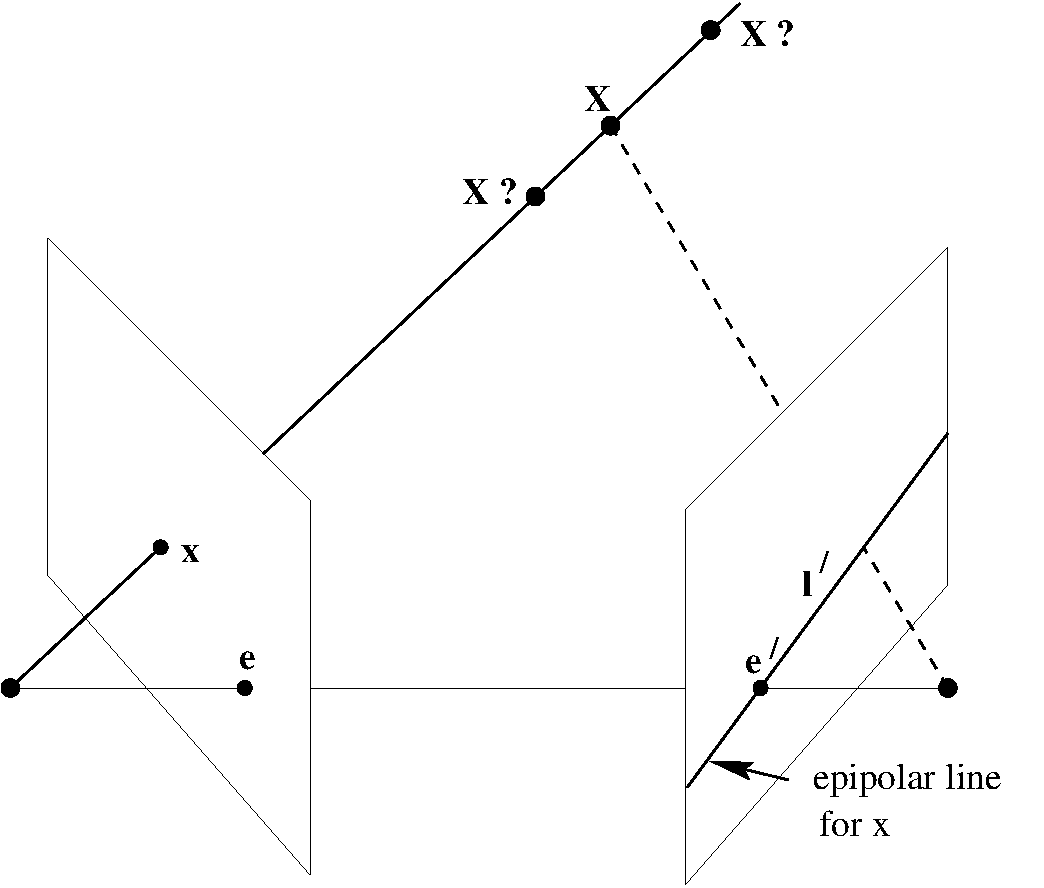
\includegraphics[width=5cm]{campair1.pdf} }}%
    \qquad
    \subfloat{{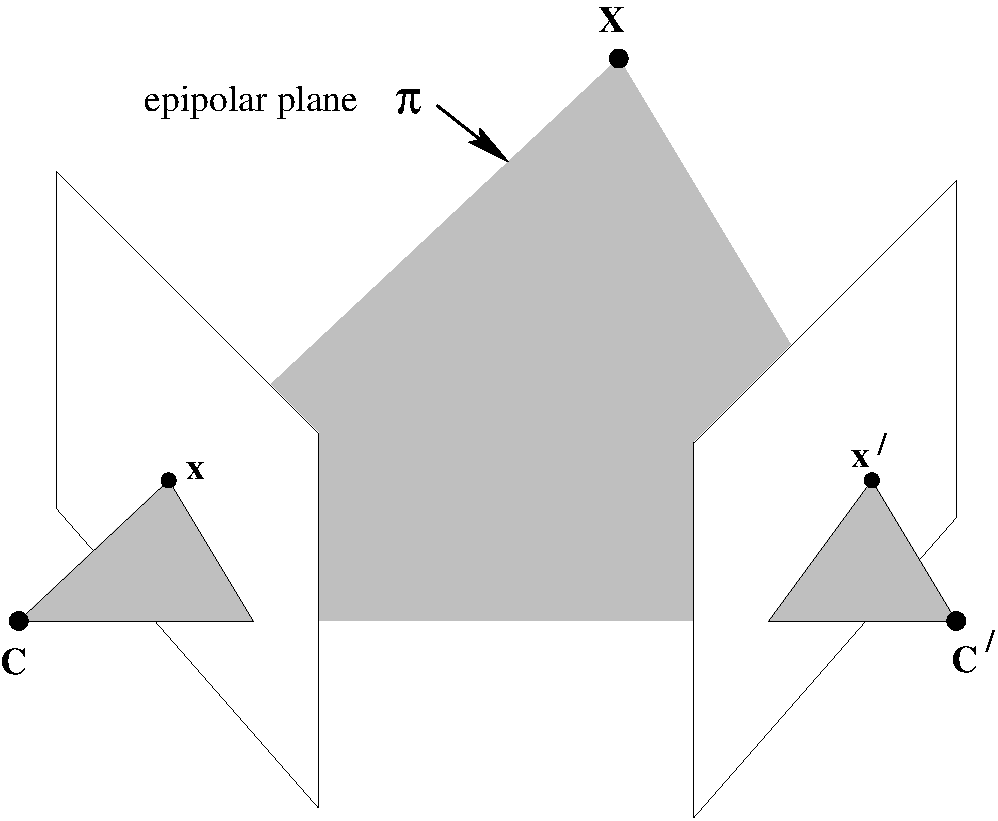
\includegraphics[width=5cm]{campair2.pdf} }}%
    \caption[Camera pair]{Camera pair. Courtesy of~\cite{HartZiss}}%
    \label{fig:campair}%
\end{figure}

Extrinsic parameters of a camera pair can be concisely given by the translation vector between camera centers $\mathbf{t}= \mathbf{C}_1-\mathbf{C}_2$ and the rotation matrix between cameras' coordinate systems $\mathtt{R}=\mathtt{R}_2\,\mathtt{R}_1^T$. If $\mathtt{R}, \mathbf{t}$ are known, extrinsics $\mathtt{R}_1, \mathtt{R}_2, \mathbf{C}_1, \mathbf{C}_2$ are defined up to a projective transformation.

Geometry of two cameras and a point in the world space seen by both cameras is usually described in terms of epipoles, which are the key concept of epipolar geometry. 


\begin{defn}
\textit{The baseline} is the line in 3D joining two camera centers.
\end{defn}

\begin{defn}
\textit{The epipole} $\mathbf{e}_i$ is the point in image plane that lies at the baseline. Equivalently, it is the point to which the center of another camera projects. 
\end{defn}

\begin{defn}
\textit{An epipolar line} $\mathbf{l}$ is a line in image plane on which the epipole of that plane lies.
\end{defn}

\begin{defn}
\textit{An epipolar plane} $\mathbf{\pi}$ is a plane in the world space which contains the line joining camera centers. The plane is associated with two epipolar lines that it contains.
\end{defn}

The information about camera epipolar geometry can be described by a single matrix as defined next. If interested, see extended discussion and proofs in \cite{HartZiss}.

\begin{defn}
\textit{An essential matrix} $\mathtt{E}$ is a matrix of the form $ \mathtt{E} = \mathtt{R} \cross{\mathbf{t}}$. The essential matrix is defined up to overall scaling.
\end{defn}

As can be seen from its construction, an essential matrix can only be of rank 2. A weaker version of this constraint can be stated as the rank constraint: 
\begin{equation}
\det{\mathtt{E}} = 0.
\label{eq:rank}
\end{equation}

The two non-zero singular values of an essential matrix are equal. This constraint can be stated as the next matrix equation (also called the trace constraint):
\begin{equation}
2 \mathtt{E} \mathtt{E}^\T \mathtt{E} - \trace{(\mathtt{E} \mathtt{E}^\T)} \mathtt{E} = 0.
\label{eq:trace}
\end{equation}

The equations \ref{eq:rank} and \ref{eq:trace} together are called  Demazure polynomials~\cite{Demazure}.

Essential matrix does not capture intrinsic camera parameters. For this purpose, the fundamental matrix is used.

\begin{defn}
\textit{The fundamental matrix} $\mathtt{F}$ corresponding to an Essential matrix $\mathtt{E}$ is given by

\begin{equation}
\mathtt{F} = \mathtt{K}_2^{-\T} \mathtt{E} \mathtt{K}_1^{-1}. 
\label{eq:fundamental}
\end{equation}
 The fundamental matrix is, like the essential matrix, defined up to overall scaling.
\end{defn}

The fundamental matrix of a camera pair defines a specific mapping from points in one image to epipolar lines in another image. Suppose that given an image point $\mathbf{x}_1 \in \Proj^3$ and two cameras $\mathtt{P}_1$, $\mathtt{P}_2$, the line $\mathbf{C}_1 \mathbf{x}_1$ in world space  is projected by the second camera to the line $\mathbf{l}_2 \in \Proj^3$ in the second camera image space. Then we can obtain $\mathbf{l}_2$ by $\mathbf{l}_2=\mathtt{F} \mathbf{x}_1$

\begin{defn}
We say that a point in one camera $\mathbf{x}_1$ and a point in another camera $\mathbf{x}_2$ form a \textit{correspondence} if there exists a 3D point $\V{X}$ that projects to $\V{x}_1$ and $\V{x}_2$.
\end{defn}

For each correspondence $\mathbf{x}_1, \mathbf{x}_2$, the fundamental matrix satisfies the so-called Epipolar constraint:
\begin{equation}
\mathbf{x}_2^\T \mathtt{F} \mathbf{x}_1 = 0.
\label{eq:epipolar}
\end{equation}

As with essential matrices, a fundamental matrix can only be of rank two. On the other hand, every matrix of rank two is a fundamental matrix~\cite{HartZiss}. A fundamental matrix satisfies the rank constraint
\begin{equation}
\det{\mathtt{F}} = 0.
\label{eq:rankF}
\end{equation}

A version of trace constraint on fundamental matrix can be formulated by substituting equation \ref{eq:fundamental} into equation \ref{eq:trace}.

\section{Computing focal lengths from point correspondences}
Given a set of points in one image $X_1$ and a set of points in another image $X_2$ that correspond to the same points $X$ in the world space, it is possible in some cases to determine the positions of points $X$ as well as intrinsic and extrinsic parameters of both cameras. This section guides the reader through the process.

Note, that in this part we assume that the point correspondences are given to us by a black box algorithm. In fact, many algorithms and modifications thereof were developed to this end, the most notable being the RANSAC family of algorithms~\cite{ransac}.


\subsection{Fundamental matrix computation}

First, we need to estimate the fundamental matrix $\mathtt{F}$ of a camera pair. In fact, all the information we need is contained in this matrix. 
Various algorithms exist that can compute the matrix $\mathtt{F}$ from point correspondences. We present two methods that are, to our best knowledge, used the most. They are relatively simple and can be implemented efficiently. 

The algorithms which we present can be formulated as so-called algebraic solvers, which work by way of constructing a set of constraints on the matrix $\mathtt{F}$ given the correspondences, and then solving the constraints in an algebraically precise way, giving all possible solutions. If the constraints are represented by polynomial equations the techniques of algebraic geometry can be used to solve these constraints.

We first define the 7pt algorithm. The algorithm uses (at least) 7 different epipolar constraints~\ref{eq:epipolar} and the rank constraint~\ref{eq:rankF}. This gives us 8 constraints on a 3$\times$3 matrix. Note, however, that all of the constraints are homogeneous polynomials, and thus the solution to the system will be a finite number\footnote{We suppose that the constraints are algebraically independent. Equivalently, at least 7 of the correspondence point pairs are in general position.} of linear one-dimensional spaces of matrices. As a fundamental matrix is defined up to scaling, this corresponds to a finite number of fundamental matrices. Moreover, the number of matrices can be expected to be no more than 3\footnote{This number is calculated as the product of degrees of the polynomials entering the system, which is  $3 \cdot 1^7$.}.

The algorithm uses SVD procedure which serves as an implicit optimization of the epipolar constraints. In case that precisely 7 epipolar constraints are given, SVD can be replaced with Gauss-Jordan elimination, and the $\mathbf{f}_1$, $\mathbf{f}_2$ vectors will be a basis of  right null space of the matrix $\mathtt{B}$. Equivalently, the matrices $\mathtt{F}_1$, $\mathtt{F}_2$ will be a basis of the pace of matrices that satisfy seven epipolar constraints.

\begin{algorithm}[H]
\SetAlgoLined 
\LinesNotNumbered
 \KwData{list of $n \geq 7$ right image points $\mathbf{x}_{1,i}$, list of the corresponding left image points $\mathbf{x}_{2,i}$}
 \KwResult{Fundamental matrix $\mathtt{F}$}
 \Begin
    {Populate matrix $\mathtt{B} \in \mathbb{R}^{n \times 9}$ with columns $\mathbf{b}_i$:  $\mathbf{b}_i \leftarrow  \vect(\mathbf{x}_{2,i} \kronecker \mathbf{x}_{1,i})$\; 
    
    Take the right singular vectors $\mathbf{f}_1, \mathbf{f}_2$ corresponding to the two smallest singular values and transform them back to matrices $\mathtt{F}_1, \mathtt{F}_2 \in \mathbb{R}^{3 \times 3}$ \;
    
    \eIf{$\det(\mathtt{F}_2)=0$}{
    \Return{ $\mathtt{F}_2$\;}
    }{
    Solve the 3rd degree polynomial in $x$: $\det(x \mathtt{F}_1 + \mathtt{F}_2)=0$, and choose the real roots $x_i$.\;
    
    \Return{ $x_i \mathtt{F}_1 + \mathtt{F}_2$\;}}
    }
 \caption{7pt}
 \label{7pt}
\end{algorithm}

Note, that we call this algorithm 7pt because the minimal number of correspondences it needs is 7. Nevertheless, any  number bigger than 7 can also be used. No smaller number of correspondences can be used, however. It can be proven that the problem  of computing fundamental matrices  with two unknown focal lengths is inherently ill-posed when less than 7 correspondences are given. The algorithm thus solves the problem using minimal possible number of correspondences.

The second algorithm doesn't use the rank constraint~\ref{eq:rankF}. Therefore, generically we expect the result to be a matrix of rank 3 and not a valid fundamental matrix. The matrix, however, "better" satisfies the epipolar constraints~\ref{eq:epipolar}, that is, it is more loyal to the data. We will compare the performance of this algorithm to 7pt in the later parts of the work. Note that this algorithm gives precisely one real solution.

\begin{algorithm}[H]
\SetAlgoLined 
\LinesNotNumbered
 \KwData{list of $n \geq 8$ right image points $\mathbf{x}_{1,i}$, list of the corresponding left image points $\mathbf{x}_{2,i}$}
 \KwResult{Fundamental matrix $\mathtt{F}$}
 \Begin
    {Populate matrix $\mathtt{B} \in \mathbb{R}^{n \times 9}$ with columns $\mathbf{b}_i$:  $\mathbf{b}_i \leftarrow  \vect(\mathbf{x}_{2,i} \kronecker \mathbf{x}_{1,i})$\;
    
    Take the right singular vector $\mathbf{f}$ corresponding to the smallest singular value and transform it back to matrix $\mathtt{F} \in \mathbb{R}^{3 \times 3}$ \;
    
    \Return{ $\mathtt{F}$\;}
    }
 \caption{8pt}
 \label{8pt}
\end{algorithm}

Note, that we call this algorithm 8pt because the minimal number of correspondences it needs is 8. Nevertheless, any  number bigger than 8 can also be used. 

\subsection{Essential matrix computation}
\label{sec:5pt}
If all calibration information is known, we can estimate essential matrix $\mathtt{E}$ instead of $\mathtt{F}$. This can be done by transforming points so that effects of intrinsic camera parameters are removed: \[\tilde{\mathbf{x}}_i = \mathtt{K}_i^{-1} \mathbf{x}_i. \]

Then the epipolar constraint \ref{eq:epipolar} is satisfied by the essential matrix with respect to the transformed points: \[
\tilde{\mathbf{x}}_2^\T \mathtt{E} \tilde{\mathbf{x}}_1 = 
 \mathbf{x}_2^\T \mathtt{K}_2^{-\T} \mathtt{E} \mathtt{K}_1^{-1} \mathbf{x}_1 = \mathbf{x}_2^\T \mathtt{F} \mathbf{x}_1 = 0. \]

The algebraic solver for the essential matrix uses the rank constraint \ref{eq:rank}, the trace constraint \ref{eq:trace}, and needs 5 point correspondences. Note that the trace constraint is a matrix equation, and therefore actually stands as more than one constraint, which explains why counting degrees of freedom seemingly fails in this case.

The construction of the solver is considerably more involved than the previous algorithms, therefore we will only refer to the papers that describe it fully.

Nister et al.~\cite{Nister5pt} show in detail how to construct an algebraic solver for this problem. The paper makes extensive use of theory of algebraic geometry \cite{Cox1,Cox2}. It is very instructing to read through the construction of this solver.

We will, however, use another solver, described by Kukelova et al. in~\cite{Zuzana5pt}. The code can be found online at \hyperref[http://cmp.felk.cvut.cz/mini/]{''http://cmp.felk.cvut.cz/mini/''}\footnote{Enter 'Polynomial eigenvalue solutions to minimal problems in computer vision' in the search field.}. This solver, contrary to the one by Nister et al., makes it possible to use an arbitrary number of correspondences, which we will take advantage of. We will refer to this solver as \textit{5pt solver}.

For those interested, Kukelova et al. give an algorithm (with source code) that  automatically creates solvers for algebraic problems~\cite{generator}.


\subsection{Focal lengths computation}
Bougnoux~\cite{Bougnoux} gives a concise formula to compute focal length from the fundamental matrix, if principal point position is known. In the next two formulae the matrix $\mathtt{I}_2$ is defined as $\mathtt{I}_2=\diag(1,1,0)$, and $\mathbf{e}_1, \mathbf{e}_2$ are the epipoles of the first and second image correspondingly. 
\begin{equation}
\label{eq:bougnoux1}
f^2_1=-\frac{\mathbf{p}^\T_2 \cross{\mathbf{e}_2} \mathtt{I}_2 \mathtt{F} \mathbf{p}_1 \mathbf{p}^\T_1 \mathtt{F}^\T \mathbf{p}_2}{\mathbf{p}^\T_2 \cross{\mathbf{e}_2} \mathtt{I}_2 \mathtt{F}^\T \mathtt{I}_2 \mathtt{F} \mathbf{p}_2}
\end{equation}

\begin{equation}
\label{eq:bougnoux2}
f^2_2=-\frac{\mathbf{p}^\T_1 \cross{\mathbf{e}_1} \mathtt{I}_2 \mathtt{F}^\T \mathbf{p}_2 \mathbf{p}^\T_2 \mathtt{F} \mathbf{p}_1}{\mathbf{p}^\T_1 \cross{\mathbf{e}_1} \mathtt{I}_2 \mathtt{F} \mathtt{I}_2 \mathtt{F}^\T \mathbf{p}_1}
\end{equation}

The second equation may be derived from the first by switching indices and transposing the $\mathtt{F}$ matrix. 

Note that it is not possible to find a focal length unless both principal points are known. As these formulae show, generically, the focal lengths are different for different principal point positions.

\subsection{Failure cases}
\label{seq:failure}
We consider the failure cases  that may occur while estimating focal length using 7pt algorithm and the Bougnoux formula.

\subsubsection{Degeneracies}
The first possible degeneracy is that the 7 epipolar constraints~\ref{eq:epipolar} are \textit{linearly dependent}. This means that the system is underconstrained and there will be generically an infinite number of solutions. A configuration of 7 correspondences which lead to such a system is said to be in singular position.

Agarwal et al., in a thorough study \cite{OnExistence}, analyze by algebraic geometry techniques a degeneration when neither of 3 solutions that 7pt algorithm gives are actually valid Fundamental matrices. It is shown in the paper that meeting the rank constraint is not enough for a matrix to be a fundamental matrix, as it needs to be of rank precisely 2. There may be a degeneracy when the matrix \textit{is of rank 1}\footnote{We suppose that algorithm does not return zero solution $\mathtt{F}=0_{3,3}$. Our formulation of the 7pt algorithm indeed does not naturally produce this solution.}. However, the constraint "is not of rank 1" cannot be expressed algebraically in an easy way and doesn't reduce the number of degrees of freedom of $\mathtt{F}$, as it only affects an infinitely small fraction of matrices. The preferable way of dealing with this degeneracy is thus to select only the valid subset of the 3 solutions given by the 7pt algorithm.

Another degeneracy may occur when the camera pair has \textit{intersecting (or parallel) optical axes}. In that case it is impossible to determine the focal lengths~\cite{KanataniClosed}. We now formulate a concise condition which describes when this can happen.

\begin{lem}
Optical axes of cameras $\mathtt{P}_1, \mathtt{P}_2$ as lines in projective $\Proj^3$ space intersect\footnote{In projective space we say that two parallel lines intersect at a point at infinity.} if and only if the principal points $\mathbf{p}_1$, $\mathbf{p}_2$ satisfy the epipolar constraint \begin{equation*}
      \mathbf{p}_2^\T \mathtt{F} \mathbf{p}_1 = 0.
\end{equation*} 

Moreover, if the principal points are zero points $\mathbf{p}_1=\mathbf{p}_2=\mat{ccc}{0 & 0 & 1}^\T$, the optical axes intersect if and only if the rightmost lowest element of the corresponding fundamental matrix $\mathtt{F}$ is zero \[ \mathtt{F}_{3,3} = 0\].
\label{interlemma}
\end{lem}

\begin{proof}
 The first part. If optical axes intersect, the point at their intersection is projected to images' principal points. Thus, principal points form a correspondence and must satisfy the epipolar constraint. Conversely, if the principal points satisfy the epipolar constraint, they must lie in an epipolar plane (see Fig. \ref{fig:campair}). The optical axes are then also lying in the epipolar plane, and each two projective lines in a plane intersect.
 
 The second part. Consider the following: \[ \mathbf{p}_2^\T \mathtt{F} \mathbf{p}_1 = \mat{ccc}{0 & 0 & 1} \mat{ccc}{
 \mathtt{F}_{1,1} & \mathtt{F}_{1,2} & \mathtt{F}_{1,3} \\ \mathtt{F}_{2,1} & \mathtt{F}_{2,2} & \mathtt{F}_{2,3} \\ \mathtt{F}_{3,1} & \mathtt{F}_{3,2} & \mathtt{F}_{3,3}}
 \mat{ccc}{0 \\ 0 \\ 1} = \mat{ccc}{0 & 0 & 1} \mat{ccc}{\mathtt{F}_{1,3} \\ \mathtt{F}_{2,3} \\ \mathtt{F}_{3,3}} = \mathtt{F}_{3,3}\]
\end{proof}

A further degeneracy \cite{HartZiss} occurs when  the plane defined by the baseline and the optical axis of one camera \textit{is perpendicular} to the plane defined by the baseline and optical axis of the other camera. In this case the Bougnoux formulae have zero denominator and thus fail to estimate the focal lengths.

\subsubsection{Invalid solutions}
There are also cases when the matrix and the focal lengths can be computed but don't correspond to any real camera configuration.

Some solutions that may need to be filtered out are \textit{complex} $\mathtt{F}$ \textit{matrices}. In the 7pt algorithm, as we are solving a 3rd degree polynomial, we may end up with 2 complex and one real solution. This might be a problem if the real solution $\mathtt{F}$ is a matrix on rank 1, and thus we don't have any valid result.

Hartley shows in~\cite{HartleyPriors} that the focal lengths computed may be imaginary, which again leads to impossible camera configuration. This happens because the focal length enter the Bougnoux formulae (Eq.~\ref{eq:bougnoux1}) only squared, so a negative estimation of $f^2$ leads to a purely imaginary focal length and can occur even when all the coefficients are real. Hartley argues that this is unacceptable and addresses the problem by developing a new algorithm to find a matrix which will have a valid focal length. 

Another problem is described in conjunction with the notion of \textit{cheirality} in~\cite{Cheirality}. In the projective camera model, we allow the points from behind the camera to be projected to image plane. This introduces an ambiguity when decomposing the essential matrix into rotation and translation. Four different camera pairs can be constructed that will have the same essential matrix, corresponding to two possible orientations of each camera, one that has points in front of it and one that has points behind.

Normally, we are able to pick the right reconstruction by selecting the camera pair such that cameras have points in front of them in world space. However, with presence of large noise it can happen that no such camera pair will exist. Usually the configuration that has the points in front of it is chosen, but this strategy can produce a wrong configuration. 

%\section{Getting point correspondences}
%for joint estimation of correspondence inlier pairs and camera parameters.


\section{Algebraic Geometry}

This section serves as a brief introduction of the topic of algebraic geometry. We follow the notation of Cox et al. from \cite{Cox1}\cite{Cox2}. We refer an interested reader to these books. 

First we define the key algebraic object of the algebraic geometry.

\begin{defn}
Given a polynomial ring $\C[x_1,x_2, \dots, x_n]$, \textit{an ideal} $I$ is such a subset of the ring that is closed under addition as well as under multiplication by a polynomial from $ \C[x_1,x_2, \dots, x_n]$. Specifically,
\begin{align*}
  & \forall f_1,f_2 \in I \; : \;  f_1+f_2 \in I \\
  & \forall f \in I, h \in  \C[x_1,x_2, \dots, x_n] \; : \; h f \in I .  
\end{align*}
\end{defn}
We can generate a geometrical object from an ideal, as outlined in the next definition.

\begin{defn}
We define a function $\textbf{V}(I)=V$, where $I \subset \C[x_1,x_2, \dots, x_n]$, and $V \subset \C^n$. \[\textbf{V}(I)=\{ a \in \C^n \; | \; f(a) = 0 \text{ for all } f \in I \} \] Intuitively, $V$ is a set of solutions to a (possibly infinite) system of polynomial equations~$I$.
\end{defn}

The geometrical sets that can be constructed in such a way are called varieties.
\begin{defn}
\textit{A variety} $V$ is such a set $V \subset \C^n$ that $\textbf{V}(I)=V$ for some system of polynomial equations  $I \subset \C[x_1,x_2, \dots, x_n]$. 
\end{defn}

We can also generate an ideal back from a variety.
\begin{defn}
We define a function $\textbf{I}(V)=I$, where $V \subset \C^n$, and $I \subset$ \( \C[x_1,x_2, \dots, x_n]\). \[\textbf{I}(V) =  \{f \in \C[x_1,x_2, \dots, x_n] \; | \; f(a) = 0 \text{ for all } a \in V \}. \] Intuitively, $I$ is a maximal set of polynomial equations that determines the geometrical set $V$.
\end{defn}

A known result~\cite{Cox1} is that $\textbf{V}(\textbf{I}(V))=V$. Under a certain assumption\footnote{When the ideal concerned is a so-called radical ideal~\cite{Cox1}.}, the opposite is also true $\textbf{I}(\textbf{V}(I))=I$.

An important notion of Gr\"obner bases is somewhat analogical to linear bases from linear algebra. Defining Gr\"obner bases requires more involved terms, so we won't do it here. Instead, we state an important result, which offers an intuitive understanding of them. 
\begin{defn}
If $G$ is \textit{a Gr\"obner basis} $G=\set{g_1, g_2, \dots, g_m} \subset I$ of an ideal \\ $I \subset \C[x_1,x_2, \dots, x_n]$, then: \[ I = \langle g_1, g_2, \dots, g_m \rangle = \{  \sum_{i=1}^m h_i g_i \; | \;  h_1, h_2, \dots, h_m \in \C[x_1,x_2, \dots, x_n] \} \]
\end{defn}

An important result~\cite{Cox1} states that every ideal defined on a finite-dimensional polynomial ring has a finite Gr\"obner basis. Continuing the analogy with linear bases, a Gr\"obner basis of a set of polynomials of degree 1 (i.e., linear equations) system is indeed its linear basis.

